\chapter{Editeur}

Pour pouvoir utiliser le logiciel de jeu existant sur d'autres morceaux, il fallait être capable de créer un document compris par le logiciel de jeu mais correspondant à d'autres musiques. Pour ce faire, nous avons créé un logiciel d'édition de morceaux, qui peut créer un fichier correspondant au format lu par le logiciel de jeu. Le format d'échange des données, qui est décrit plus bas, nous a donc imposé de diviser la partie éditeur en deux. Chronologiquement, une première partie où l'utilisateur saisit les accords à jouer et une deuxième où il indique les moments auxquels il faut les jouer.

\section{Format d'échange}

Le format d'échange entre le logiciel de jeu et le logiciel d'édition est le même que celui qu'utilisait auparavant le logiciel de jeu.
En voici un exemple :
\begin{verbatim}
[INTRO]
1.914761 G
1.455219 Bm
3.149589 Em
6.328478 C
[VERSE1]
1.577916 G
1.497687 Bm
1.567347 Em
\end{verbatim}
Comme nous pouvons le voir, deux ou trois éléments le compose :
\begin{itemize}
\item des annotations entre crochets
\item les notes à jouer
\item la durée de la note, qui correspond au temps entre deux notes
\end{itemize}
Pour répondre à ce format, nous avons séparés la saisie des notes et des annotations dans la première partie et la saisie des intervalles de temps dans la seconde.

\section{Saisie des notes}

\subsection{Le logiciel}

Tout d'abord, l'utilisateur commence par entrer les accords dans une grille dédiée. Il y a la possibilité de faire varier le nombre de ligne et de colonne de cette grille. En plus des colonnes d’accords il y en a une d’annotations.

Le choix du nombre de colonnes se fait au moment de la création d’une nouvelle grille grâce au bouton "new". Le nombre de lignes, lui, peut être modifié à la volée en insérant des lignes à l’endroit souhaité.

Pour remplir les cases avec des notes, vous devez sélectionner une ou plusieurs cases, et choisir ensuite dans la liste hiérarchique de gauche l’accord que vous souhaitez en double cliquant dessus. En cliquant sur les fondamentales de la liste d’accords, les variantes vous sont affichées.
Les cases d’annotations sont des cases de texte libre permettant de renseigner les informations souhaités par l'utilisateur. \\

Plusieurs manipulations de la grille d'accords sont possibles. Il est possible de supprimer une ou plusieurs lignes en les sélectionnant, puis en cliquant sur le bouton "delete row" à droite.
Il est possible de copier la ligne ou un bloc de ligne vers le bas. Il faut sélectionner le bloc souhaité et utiliser le bouton "Copy down". Les nouvelles lignes sont insérées en dessous du bloc sans modifier le reste de la grille. \\

Le bouton "Save" permet de sauvegarder la grille courante, terminée ou non, au format \textit{xgrid}. La sauvegarde se fait dans le répertoire par défaut. Si la grille n’a pas encore été nommée, il faut alors lui donner un nom avant la sauvegarde.
Le bouton "Open" permet de choisir une grille au format xgrid et de l’ouvrir, elle peut ensuite être modifiée. \\

Voici une capture d'écran illustrant la fenêtre intégrant cette grille d'accords et les boutons en question:
\begin{figure}[!h]
\begin{center}
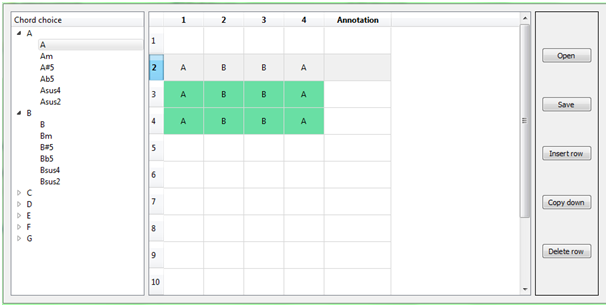
\includegraphics[scale=0.5]{grilleAccordBloc.png}
\end{center}
\caption{Interface de saisie des notes}
\end{figure}
 
\subsection{La sauvegarde des grilles}

Pour sauvegarder les grilles d'accords, elle sont exportées en XML avec une extension \textit{xgrid}. Ce fichier contient toutes les informations nécessaire à la construction d'une grille :

\begin{enumerate}
\item{Le nom} de la grille.
\item{Le nombre de lignes et de colonnes} de la grille.
\item{Les accords} contenus dans chaque case.
\item{Les annotations} de chaque ligne.
\end{enumerate}~

Voilà l'exemple d'une grille ainsi que le fichier xgrid qui lui correspond.

\begin{figure}[H]
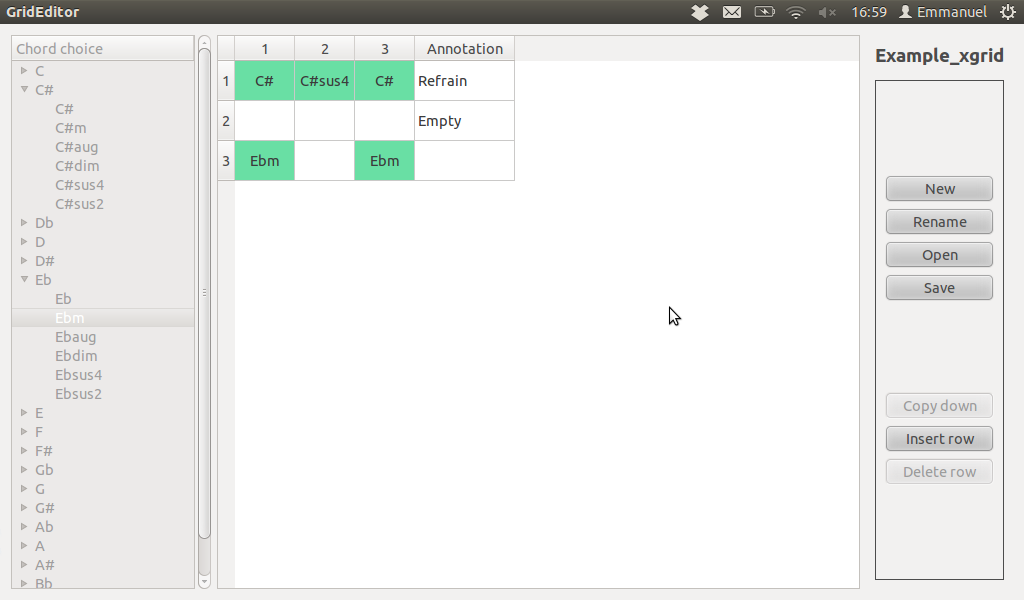
\includegraphics[width=\textwidth]{grid_example.png}
\caption{Exemple de grille d'accords.}
\label{grid_example}
\end{figure}

Le fichier xgrid correspondant à l'image \ref{grid_example}.

\begin{verbatim}                                                                                          
<!DOCTYPE XGRID>
<chord_grid lines_number="3" columns_number="4" name="Example_xgrid">
 <line id="0">
  <case id="0">
   <chord name="C#"/>
   <color G="200" R="0" A="150" B="100"/>
  </case>
  <case id="1">
   <chord name="C#sus4"/>
   <color G="200" R="0" A="150" B="100"/>
  </case>
  <case id="2">
   <chord name="C#"/>
   <color G="200" R="0" A="150" B="100"/>
  </case>
  <annotation>Refrain</annotation>
 </line>
 <line id="1">
  <case id="0">
   <chord name=""/>
   <color G="255" R="255" A="255" B="255"/>
  </case>
  <case id="1">
   <chord name=""/>
   <color G="255" R="255" A="255" B="255"/>
  </case>
  <case id="2">
   <chord name=""/>
   <color G="255" R="255" A="255" B="255"/>
  </case>
  <annotation>Empty</annotation>
 </line>
 <line id="2">
  <case id="0">
   <chord name="Ebm"/>
   <color G="200" R="0" A="150" B="100"/>
  </case>
  <case id="1">
   <chord name=""/>
   <color G="255" R="255" A="255" B="255"/>
  </case>
  <case id="2">
   <chord name="Ebm"/>
   <color G="200" R="0" A="150" B="100"/>
  </case>
  <annotation></annotation>
 </line>
</chord_grid>                                                                            
\end{verbatim}


\section{Saisie des temps}
Une fois la saisie des notes réalisée, l'utilisateur accède à une seconde vue pour réaliser la saisie des temps. Voici l'interface qu'aperçoit l'utilisateur :
\begin{figure}[!h]
\begin{center}
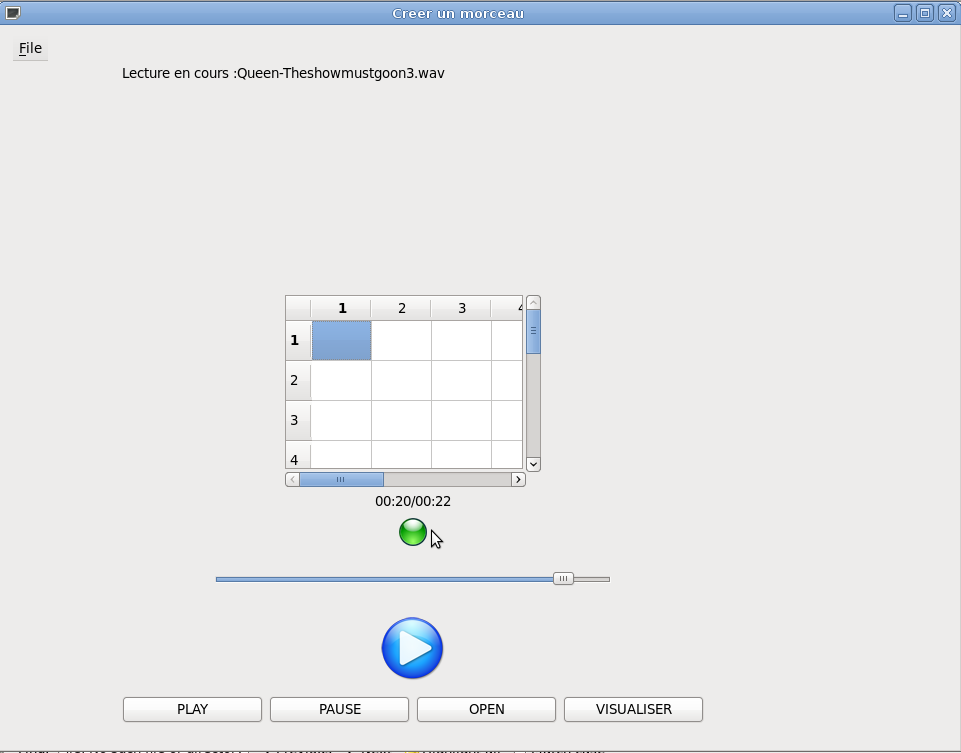
\includegraphics[scale=0.5]{editeur.png}
\end{center}
\caption{Interface de saisie des temps}
\end{figure}
Nous pouvons observer, de haut en bas:
\begin{itemize}
\item nom de la piste en lecture
\item accords précédemment saisis pour lesquels il faut saisir un temps
\item la position dans la musique
\item un icone représentant l'état actuel de la musique (en cours, en pause)
\item les trois boutons pour gérer la lecture de la musique ainsi que le bouton pour passer en mode visualisation
\end{itemize}
\subsection{fonctionnement}

\indent Afin de réaliser le fichier texte correspondant à la musique que l'on veut créer, l'utilisateur commence par sélectionner le fichier wav lui correspondant. Nous avons implémenté trois manières d'ouvrir un fichier :
\begin{itemize}
\item à partir de la barre de menu file -> ouvrir une musique
\item en utilisant le raccourci clavier Ctrl + o
\item en appuyant sur le bouton \textbf{ouvrir}
\end{itemize}

\indent Une fois la musique chargée, l'utilisateur dispose des fonctionnalités d'un lecteur classique, c'est-à-dire la lecture, la pause ainsi que le déplacement dans la musique en déplacant le curseur de la barre d'avancement. Il peut, bien entendu, également changer de musique en réutilisant la barre des menus ou le raccourci Ctrl + o.
\\
\indent La deuxième fonctionnalité majeure est la saisi des temps où il faut jouer les accords. Pour cela, l'utilisateur doit, tout en écoutant la musique, appuyer sur la barre espace pour saisir un temps. Si l'utilisateur se trompe, il peut revenir en arrière avec le curseur de la barre d'avancement qui aura pour effet de supprimer toutes les saisies postérieures à la nouvelle postion du curseur dans la musique.
\\
\indent Enfin il exsite un mode de visualisation pour voir les temps saisis. Pour l'activer, il suffit de cliquer sur le bouton Visualisation, la saisie des temps sera toujours possible, mais le déplacement dans la musique ne supprime plus les temps saisies. Pour le quitter il suffit simplement de cliquer sur le bouton Stop Visualisation.
\\
\indent Enfin lorsque l'utilisateur est satisfait des temps et des accords saisis, il lui suffit d'exporter les données dans le format voulu en utilisant la barre des menus ou le raccourci Ctrl + e.

\subsection{implémentation}
\indent Pour réaliser cette partie, le code a été divisé en deux. Une première classe se chargeant de la partie lecture audio et saisi des temps et une deuxième qui s'occupe de la phase de visualisation.
\\
\indent Lors de la création d'un nouveau morceaux, la classe createwindow se charge d'instancier un objet player, qui correspont à la première partie cité ci-dessus, et de connecter les signaux aux méthodes. Ensuite c'est l'instance du player qui se charge de créer un visualisationthread dès lors que l'utilisateur souhaite visualiser ce qu'il a déjà saisi.
\\
Enfin pour aider l'utilisateur une barre des menus QMenuBar reste à disposition.
\subsection{correspondance avec les demandes du client}

\indent La partie lecture audio n'ayant pas été abordé avec le client, nous nous sommes contentés des fonctionnalités de base, contrairement à la saisi des temps par la barre espace qui avait été discuté et dont nous avions trouvé accord. Un retour visuel et une visualisation possible de ce qui a été fait a été ajouté pour permettre une meilleur utilisation.

\section{Evaluation cognitive}

\indent Après la mise en place de l'éditeur, nous avons essayé d'évaluer qualitativement l'interface de celui-ci mettant en oeuvre des techniques de cognitique utiles à l’évaluation ergonomique d’une interface. Nous avons centré la validation de notre
interface sur un nombre limité de critères ergonomiques dont l’évaluation se fera d’une part avec une évaluation analytique : la Balade cognitive, et d’autre part avec une évaluation expérimentale : les tests utilisateurs.

\begin{itemize}

\item La balade cognitive :  Nous avons essayé d'imaginer tous les scénarii possibles pour la création d'un morçeau. Par la suite, nous avons effectué des modifications sur l'interface en prenant en considération les problèmes rencontrés.
\item Les tests utilisateurs : Nous avons créé un recette de test utilisateurs. Ensuite, nous avons déroulé le scénario test
``création d'un morceau`` en invitant un élève de l'ENSEIRB-MATMECA à utiliser le logiciel éditeur.
\end{itemize}

Enfin, nous nous sommes intéressés à l’évaluation de cette expérimentation et finir par effectuer des modifications sur l'interface, notemment sur la dénomination des boutons.
